\documentclass[UTF8]{article}
\usepackage{graphicx}
\usepackage{indentfirst}
\usepackage{subfigure}
\usepackage[UTF8]{ctex}
\usepackage{amsmath}
\usepackage{enumitem}
\usepackage{geometry}
\usepackage{float}
\usepackage{wrapfig}
\usepackage{setspace}

\geometry{a4paper,left=1.5cm, right=1.5cm, top=1.7cm, bottom=1.7cm}

\title{利用相对运动处理外力不平衡时的磁场运动}
\author{千丛恋雨万花绫}
\date{2022年 3月 27日}

\begin{document}

\maketitle

\setstretch{lineSpread}

本笔记讨论点电荷在磁场中所受外力不平衡,且不与洛伦兹力平衡的情况

\section*{引}

此类情况下点电荷的运动属于竞赛知识,高考中不常见。但此类问题并非没有考过,最典型的有2008年江苏卷,2015年福建卷。

记 $F_{B}(v)$ 为速度 $v$ 产生的洛伦兹力,有 $F_{B}(v)=Bqv$

由于$Bq(v_{1}+v_{2}=Bqv_{1}+Bqv_{2}$,显然有$F_{B}(v_{1}+v_{2})+F_{B}(v_{1})+F_{B}(v_{2})$

\section*{知识点\ 相对运动}

动点相对于静止参考系的速度称为绝对(absolute)速度,记作$v_{a}$.一般来说,选定地面为静止参考系。在研究相对运动时,一般只研究质点,不研究刚体。因为相对运动下的刚体运动过于复杂。

选定静止参考系后,选定任一参考系为动参考系,该参考系可以按需自由定义。

动参考系任意一点相对静止参考系的速度有时是无法确定的,比如动参考系转动时,各点的速度不同。本笔记中只会出现动参考系相对静参考系平动(无转动)且匀速直线运动的情况。

\begin{wrapfigure}{l}{0.23\textwidth}
    \centering
    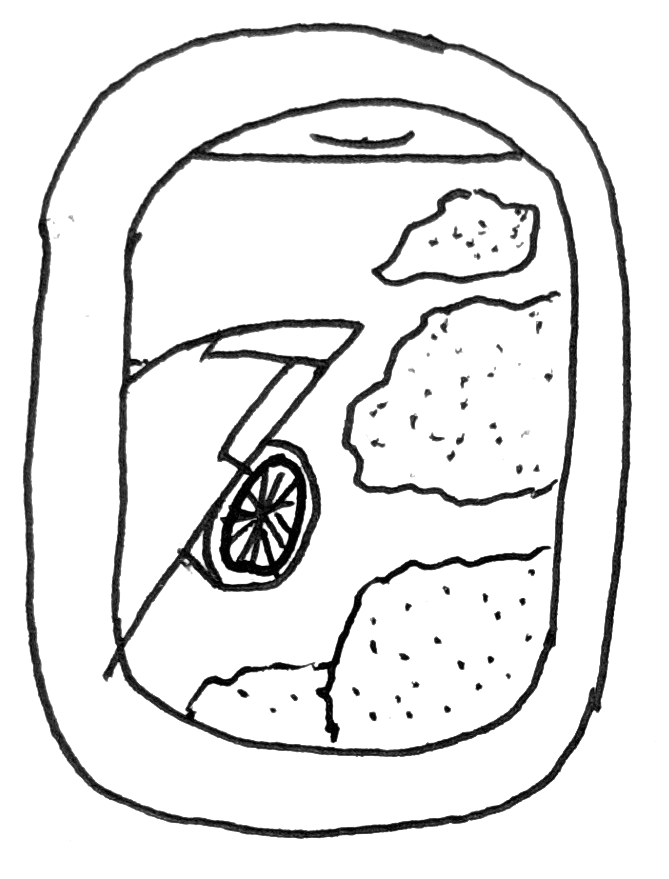
\includegraphics[width=0.2\textwidth]{onPlane}
    \caption{飞机窗外}
\end{wrapfigure}

记动参考系任意一点相对静参考系的速度为牵连(transfer)速度,记作$v_{e}$.记动点相对动参考系的速度为相对(relative)速度,记作$v_{r}$

如图1,想象你在一个匀速直线运动的飞机上,选定地面为静参考系,飞机为动参考系,云朵上的某一点相对于你的速度为$v_{r}$,相对于地面的速度为$v_{a}$,而飞机相对于地面的速度为$v_{e}$,不难理解:

\[v_{a}=v_{e}+v_{r}\]

另外,当动参考系做匀速直线运动时,可以将静参考系上的力不加变换而直接移到动参考系上,因为牛顿第二定律无关于参考系。如果动参考系不是匀速直线运动,则不行,因为此时动参考系不符合牛顿运动定律。

\section*{核心知识\ 配速法}

\begin{wrapfigure}{l}{0.33\textwidth}
    \centering
    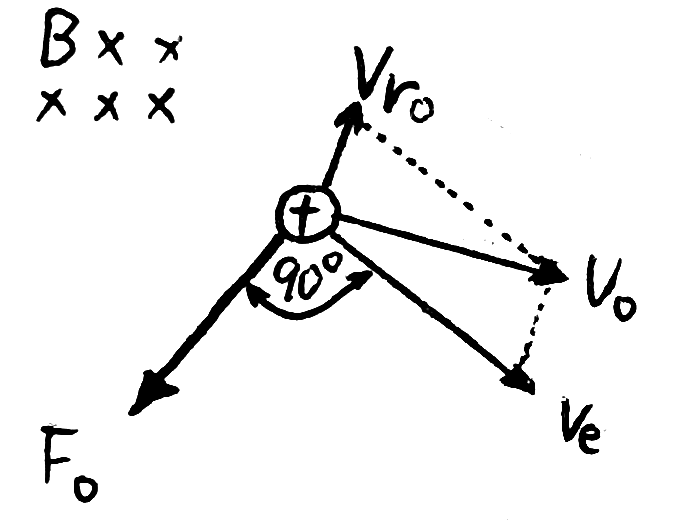
\includegraphics[width=0.3\textwidth]{vArrange.png}
\end{wrapfigure}

如图,一正电荷在垂直于纸面向内的磁场中,受到除洛伦兹力的恒定合外力$F_{0}$,初速度为$v_{0}$.

令$F_{B}(v_{e})=-F_{0}$,即$v_{e}=- \frac{F_{0}}{Bq}$

将$v_{0}$分解为$v_{r0}$和$v_{e}$,于是就可以分解正电荷所受库仑力

\[F_{B}(v_{a})=F_{B}(v_{e}+v_{r})=F_{B}(v_{e})+F_{B}(v_{r})\]

\ 

如此,就有所受合力为

\[F_{\text{合}}=F_{0}+F_{B}(v_{a})=F_{0}+F_{B}(v_{e})+F_{B}(v_{r})\]

由于$F_{B}(v_{e})=-F_{0}$,得

\[F_{\text{合}}=F_{B}(v_{r})\]

由于动参考系以$v_{e}$匀速直线运动,牛顿运动定律适用于动参考系,静参考系中的力可以直接移到动参考系中,并产生相对两个参考系相同的加速度。于是,相对于动参考系,正电荷始终只受到一个使它匀速圆周运动的洛伦兹力。也就是说,正电荷相对动参考系匀速圆周运动,且速度为$v_{r}$

由$v_{a}=v_{e}+v_{r}$,我们可以得出:正电荷相对静参考系做匀速圆周运动和匀速直线运动的合运动

\section*{运动的轨迹}

显然,轨迹形状取决于$v_{e}$和$v_{r}$

若$v_{0}=0$,则$v_{r0}=\frac{F_{0}}{Bq}$,与动参考系速度相同,此时轨迹为摆线(下图a)

\begin{figure}[H]
    \centering
    \subfigure[摆线]{%
    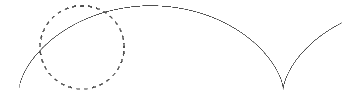
\includegraphics[width=0.25\textwidth]{swin.png}
    \label{fig:subfigure1}
    }
    \subfigure[短摆线]{%
    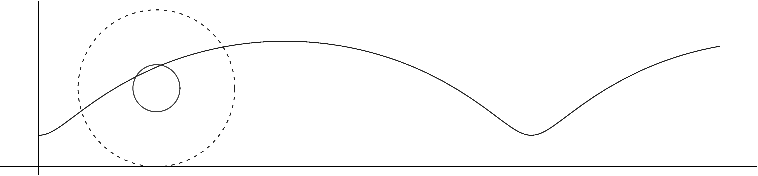
\includegraphics[width=0.3\textwidth]{shortSwin.png}
    \label{fig:subfigure2}
    }
    \subfigure[长摆线]{%
    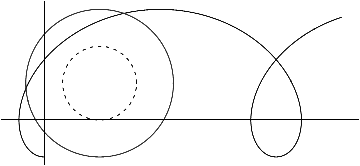
\includegraphics[width=0.25\textwidth]{longSwin.png}
    \label{fig:subfigure3}
    }
    \caption{三种轨迹}
\end{figure}

可以通过下图a的滚胶带实验理解摆线

\begin{figure}[htbp]
    \centering
    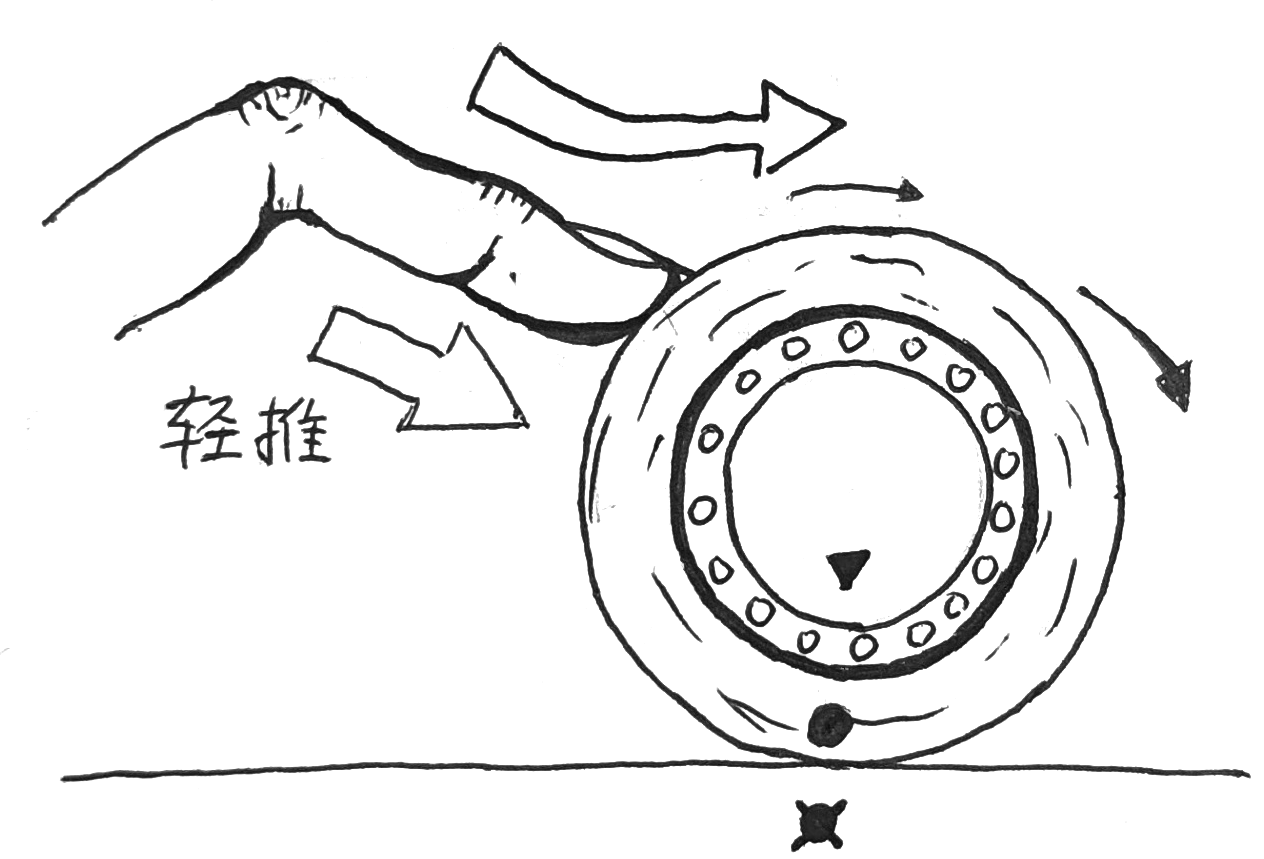
\includegraphics[width=0.5\textwidth]{roll.png}
    \caption{滚胶带实验}
\end{figure}

在胶带尽可能边缘处打上一个点(图中圆点),让胶带竖直立于桌面,并使点位于正下方。轻推胶带,使其滚动,圆点的轨迹即为摆线。

若初速度不为0,则轨迹不是摆线,而是长摆线或短摆线。

若$r=\frac{mv_{r}}{Bq} < \frac{mv_{e}}{Bq}$,也就是$v_{r} < v_{e}$时,标记点在胶带内(图中三角点)。轨迹如图b,其中虚线为胶带边缘。

若$v_{r} > v_{e}$,标记点在胶带外(图中圆叉点)。轨迹如图c,其中虚线为胶带边缘。

\end{document}
